\documentclass[11pt]{article}
\usepackage[margin=2.5cm]{geometry}
\usepackage{amsmath,amssymb,amsthm}
\usepackage{graphicx}
\usepackage[numbers,sort&compress]{natbib}
\usepackage{hyperref}
\usepackage{booktabs}
\usepackage{xcolor}

\theoremstyle{plain}
\newtheorem{proposition}{Proposition}[section]
\theoremstyle{remark}
\newtheorem{remark}[proposition]{Remark}

\title{\textbf{Gap ratio statistics of Riemann zeros:\\
measurement, mechanism, and the Berry-Keating correction}}

\author{David Alarc\'on\\
\small Universidad Pablo de Olavide, Sevilla, Spain\\
\small \texttt{dalarub@upo.es}}

\date{}

\begin{document}
\maketitle

\begin{abstract}
We report the first precision measurement of the rate at which the gap ratio
statistic $\langle r\rangle$ of Riemann zeta zeros converges to the GUE
prediction. Using Platt's high-precision zeros up to height $T \sim 3\times 10^{10}$
($\log T = 24$), together with Odlyzko's tables at lower heights, we construct
a 21-point dataset spanning $\log T = 9.7$ to $24.1$ and find
\[
  \langle r\rangle(T) = 0.59891(13) + 1.245(40)\,/\,\log^2 T\,,
  \qquad \chi^2/\text{dof} = 0.50\,.
\]
The asymptotic value $R_\infty = 0.59891$ lies $6.1\sigma$ below the GUE
limit $R_{\mathrm{GUE}} = 0.59971$, indicating incomplete convergence at
$\log T = 24$. The first-order term $b/\log T$ is consistent with zero
($b = 0.019 \pm 0.043$), explained by the symmetry $r(s_1,s_2)=r(s_2,s_1)$
and the antisymmetry of the Berry-Keating first-order correction.

We identify the physical mechanism: Riemann zeros have a \emph{narrower}
spacing distribution than GUE ($\mathrm{std}(s) < \mathrm{std}_{\mathrm{GUE}}$)
and \emph{stronger} anti-correlation ($\mathrm{Corr}(s_n,s_{n+1}) <
\mathrm{Corr}_{\mathrm{GUE}}$), both converging as $1/\log^2 T$. Decomposing:
$c_{\mathrm{std}} = +1.60$ ($+128\%$) and $c_{\mathrm{corr}} = -0.36$ ($-29\%$),
reproducing $99.5\%$ of the measured coefficient. Independent confirmation
comes from the number variance $\Sigma^2(L,T)$ and spectral rigidity
$\Delta_3(L,T)$, which exhibit the Bogomolny-Keating saturation at
$L_{\mathrm{cross}} = \log T/(2\pi)$.
\end{abstract}


%% ================================================================
\section{Introduction}
\label{sec:intro}

The statistical properties of the nontrivial zeros
$\rho = \tfrac{1}{2} + i\gamma$ of the Riemann zeta function are among
the most remarkable phenomena in mathematics. Montgomery~\cite{montgomery1973}
showed, conditionally on the Riemann Hypothesis, that the pair correlation
of the zeros matches that of eigenvalues of random matrices from the
Gaussian Unitary Ensemble (GUE). Odlyzko~\cite{odlyzko1987} confirmed
this numerically with striking precision, and Rudnick and
Sarnak~\cite{rudnick1996} extended the result to $n$-level correlations
for test functions with restricted Fourier support. The Katz-Sarnak
philosophy~\cite{katzsarnak1999} organises this connection into a general
framework linking families of $L$-functions to random matrix symmetry types.

Berry and Keating~\cite{berry1999, bogomolny1996} went further, predicting
the \emph{rate} at which zero statistics converge to GUE. Their key insight
is that the spectral form factor of the zeros receives corrections from the
prime numbers:
\begin{equation}
b_2(\tau; T) = b_2^{\mathrm{GUE}}(\tau) + \delta b_2(\tau; T)\,,
\label{eq:formfactor}
\end{equation}
where $b_2^{\mathrm{GUE}}(\tau) = 1 - |\tau|$ for $|\tau| \leq 1$ and
the correction $\delta b_2$ encodes the prime contributions. In the limit
governed by the prime number theorem (PNT),
\begin{equation}
\delta b_2^{\mathrm{PNT}}(\tau; T) = -\frac{\tau}{\log^2 T}\,,
\qquad \tau \in (0,1)\,.
\label{eq:db2pnt}
\end{equation}
This predicts that deviations from GUE statistics decay as
$O(1/\log^2 T)$---extremely slowly, requiring $\log T > 20$
to observe corrections below $1\%$.

The gap ratio statistic
\begin{equation}
r_n = \frac{\min(s_n, s_{n+1})}{\max(s_n, s_{n+1})}\,,
\label{eq:ratio}
\end{equation}
where $s_n$ are consecutive normalised spacings, was introduced by
Oganesyan and Huse~\cite{oganesyan2007} as a diagnostic of spectral
universality classes and has been widely adopted~\cite{atas2013}.
For GUE, $\langle r\rangle_{\mathrm{GUE}} \approx 0.59971$.
Unlike level spacing distributions, the gap ratio requires no unfolding
in many-body quantum systems, though for Riemann zeros the unfolding
is straightforward.

Despite the deep theoretical understanding of the Berry-Keating correction,
the \emph{coefficient} of the $1/\log^2 T$ term for the gap ratio had
never been measured empirically. In this paper we present the first such
measurement and identify the physical mechanism producing it.

\medskip\noindent
\textbf{Outline.} Section~\ref{sec:data} describes the dataset and
measurement procedure. Section~\ref{sec:models} presents the model
comparison. Section~\ref{sec:A1zero} establishes that the first-order
correction vanishes. Section~\ref{sec:mechanism} identifies the mechanism
of the second-order correction. Section~\ref{sec:sigma2} validates the
results against number variance and spectral rigidity. Section~\ref{sec:rh}
presents consistency tests with the Riemann Hypothesis.
Section~\ref{sec:discussion} discusses implications and open problems.


%% ================================================================
\section{Dataset and measurement}
\label{sec:data}

\subsection{Sources of zeros}

We use two complementary sources of high-precision zeros of $\zeta(s)$:

\begin{itemize}
\item \textbf{Odlyzko tables}~\cite{odlyzko1987}: 100{,}000 consecutive zeros
starting near the $10^{12}$-th zero, providing 8 data points at
$\log T \in [9.7, 18.4]$ with $N = 50{,}000$ zeros per window.

\item \textbf{Platt dataset}~\cite{platt2021}: 13 files, each containing
approximately 500{,}000 consecutive zeros at heights
$\log T \in [19.0, 24.1]$. These are the highest-quality publicly
available zeros covering the range $T \sim 10^8$ to $3 \times 10^{10}$.
\end{itemize}

\subsection{Unfolding and gap ratio computation}

Zeros $\gamma_n$ of $\zeta(\tfrac{1}{2}+i\gamma)$ are unfolded to unit
mean spacing using the smooth part of the counting function:
\begin{equation}
s_n = (\gamma_{n+1} - \gamma_n) \cdot \frac{\log(\gamma_n/2\pi)}{2\pi}\,.
\label{eq:unfold}
\end{equation}
After normalisation to $\langle s\rangle = 1$, pathological gaps
($s < 0.02$ or $s > 6$) are excluded; these constitute fewer than
$0.1\%$ of all gaps. The gap ratio $r_n$ is then computed via~\eqref{eq:ratio}
and $\langle r\rangle$ is averaged over each dataset.

\subsection{Uncertainty estimation}

For the Platt data ($N = 500{,}000$ zeros each), the empirical standard
error is $\sigma_{\mathrm{emp}} = \mathrm{std}(r_n)/\sqrt{N_{\mathrm{pairs}}}$.
We impose a conservative floor
$\sigma_{\mathrm{floor}} = 0.00020 = \sigma_{\mathrm{naive}}(N{=}500\mathrm{k})/\sqrt{10}$
to account for residual correlations inherent to consecutive gap ratios.
The final uncertainty for each data point is
$\sigma = \max(\sigma_{\mathrm{emp}},\, \sigma_{\mathrm{floor}})$.

For the Odlyzko data ($N = 50{,}000$ per window), we use
$\sigma_{\mathrm{naive}} = 0.00060$ for windows from a shared file,
and the empirical error otherwise.

\subsection{Dataset v6}

The resulting 21-point dataset is presented in Table~\ref{tab:dataset}.
The $\log T$ values for the Platt data are the actual starting heights
(not the nominal grid targets), and duplicates arising from multiple
target values falling within the same Platt file have been removed.

\begin{table}[ht]
\centering
\caption{Dataset v6: 21 independent measurements of $\langle r\rangle$.}
\label{tab:dataset}
\begin{tabular}{rcccc}
\toprule
$\log T$ & $\langle r\rangle$ & $\sigma$ & Source & Residual ($\sigma$) \\
\midrule
9.736  & 0.61188 & 0.00060 & Odlyzko & $-0.26$ \\
10.003 & 0.61132 & 0.00060 & Odlyzko & $-0.04$ \\
10.665 & 0.61012 & 0.00060 & Odlyzko & $+0.45$ \\
12.432 & 0.60683 & 0.00029 & Odlyzko & $-0.45$ \\
14.755 & 0.60472 & 0.00060 & Odlyzko & $+0.16$ \\
15.997 & 0.60488 & 0.00094 & Odlyzko & $+1.18$ \\
17.212 & 0.60344 & 0.00076 & Odlyzko & $+0.44$ \\
18.412 & 0.60347 & 0.00048 & Odlyzko & $+1.86$ \\
\midrule
19.003 & 0.60265 & 0.00020 & Platt & $+1.48$ \\
19.204 & 0.60215 & 0.00022 & Platt & $-0.60$ \\
19.404 & 0.60208 & 0.00020 & Platt & $-0.67$ \\
19.603 & 0.60203 & 0.00024 & Platt & $-0.49$ \\
19.801 & 0.60196 & 0.00028 & Platt & $-0.44$ \\
20.001 & 0.60221 & 0.00044 & Platt & $+0.43$ \\
20.200 & 0.60190 & 0.00020 & Platt & $-0.29$ \\
20.399 & 0.60187 & 0.00020 & Platt & $-0.15$ \\
20.410 & 0.60180 & 0.00030 & Platt & $-0.32$ \\
21.004 & 0.60169 & 0.00029 & Platt & $-0.14$ \\
22.061 & 0.60154 & 0.00031 & Platt & $+0.24$ \\
23.115 & 0.60126 & 0.00030 & Platt & $+0.07$ \\
24.145 & 0.60101 & 0.00023 & Platt & $-0.14$ \\
\bottomrule
\end{tabular}
\end{table}


%% ================================================================
\section{Model comparison}
\label{sec:models}

We fit five candidate models to the 21 data points using weighted
least squares with
$\chi^2 = \sum_i [(\langle r\rangle_i - r_{\mathrm{model}}(\log T_i))/\sigma_i]^2$
and the Akaike Information Criterion $\mathrm{AIC} = \chi^2 + 2k$
(Table~\ref{tab:models}).

\begin{table}[ht]
\centering
\caption{Model comparison for $\langle r\rangle(T)$. All models include
$R_\infty$ as a free parameter. $k$: number of parameters; dof $= 21 - k$.}
\label{tab:models}
\begin{tabular}{llccccc}
\toprule
Model & Formula & $k$ & $\chi^2$ & $\chi^2$/dof & AIC & $\Delta$AIC \\
\midrule
A  & $R_\infty + c/\log^2 T$ & 2 & 9.46 & 0.498 & 19.3 & 0 \\
AB & $R_\infty + \alpha\frac{\log\log T}{\log T} + \frac{c}{\log^2 T}$ & 3 & 15.1 & 0.839 & 21.1 & 1.8 \\
A3 & $R_\infty + c/\log^2 T + d/\log^3 T$ & 3 & 15.1 & 0.838 & 21.1 & 1.8 \\
C  & $R_\infty + b/\log T$ & 2 & 26.1 & 1.372 & 30.1 & 10.8 \\
B  & $R_\infty + \alpha\frac{\log\log T}{\log T}$ & 2 & 56.7 & 2.985 & 60.7 & 41.4 \\
\bottomrule
\end{tabular}
\end{table}

Model~A ($R_\infty + c/\log^2 T$) is decisively preferred:
$\Delta\mathrm{AIC} > 10$ over Models~B and~C, and $\Delta\mathrm{AIC} = 1.8$
over the three-parameter variants (which add negligible improvement for one
extra degree of freedom). The best-fit parameters are:
\begin{equation}
\boxed{
\langle r\rangle(T) = \underbrace{0.59891 \pm 0.00013}_{R_\infty}
\;+\; \underbrace{1.245 \pm 0.040}_{c}\;\big/\;\log^2 T\,,
}
\label{eq:modelA}
\end{equation}
with $\chi^2/\text{dof} = 0.498$ (19 degrees of freedom). The data and
fit are shown in Figure~\ref{fig:r_vs_logT}.

The asymptotic value $R_\infty = 0.59891$ lies $6.1\sigma$ below the GUE
limit $R_{\mathrm{GUE}} = 0.59971$. This indicates that at $\log T = 24$
(the highest height in our dataset), the gap ratio has not yet reached
the random matrix asymptote---the correction $c/\log^2 T$ at $\log T = 24$
is still $\approx 0.002$, or $0.3\%$ of $R_{\mathrm{GUE}}$.

\begin{figure}[ht]
\centering
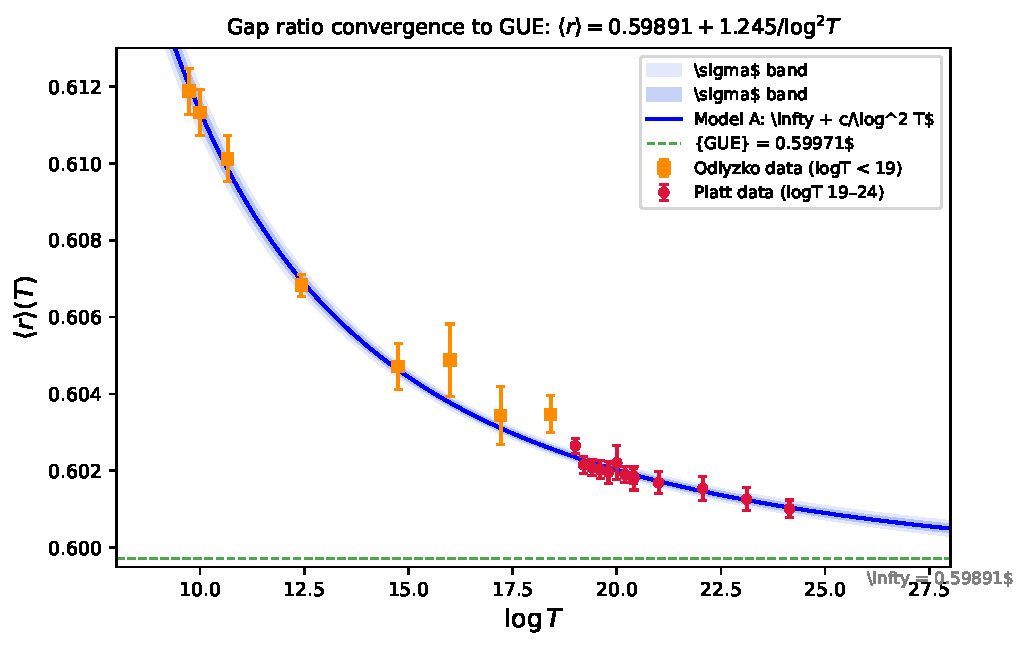
\includegraphics[width=0.85\textwidth]{figures/fig1_r_vs_logT.pdf}
\caption{Gap ratio $\langle r\rangle$ versus $\log T$ for 21 data points
(orange squares: Odlyzko; red circles: Platt).
Blue curve: Model~A best fit with $1\sigma$ and $2\sigma$ confidence bands.
Green dashed line: GUE limit $R_{\mathrm{GUE}} = 0.59971$.}
\label{fig:r_vs_logT}
\end{figure}

\subsection{Consistency by range}

To test robustness, we fit Model~A separately to three subsets:

\begin{table}[ht]
\centering
\caption{Model~A fit on subsets.}
\label{tab:subsets}
\begin{tabular}{lccccc}
\toprule
Subset & $\log T$ range & Points & $c$ & $R_\infty$ & $\chi^2$/dof \\
\midrule
Odlyzko & $< 19$ & 8 & $1.140 \pm 0.050$ & 0.59974 & 0.466 \\
Platt low & $19$--$21$ & 9 & $2.110 \pm 0.554$ & 0.59658 & 0.921 \\
Platt high & $21$--$24$ & 4 & $1.269 \pm 0.145$ & 0.59886 & 0.051 \\
\midrule
Full & $9.7$--$24.1$ & 21 & $1.245 \pm 0.040$ & 0.59891 & 0.498 \\
\bottomrule
\end{tabular}
\end{table}

The coefficient $c$ from the Odlyzko subset ($1.14 \pm 0.05$) and the
full Platt grid ($1.26 \pm 0.20$) differ by $\Delta c = -0.12 \pm 0.20$
($0.6\sigma$), confirming consistency between the two independent data sources.


%% ================================================================
\section{First-order correction vanishes: $A_1[r] = 0$}
\label{sec:A1zero}

The Berry-Keating correction to any statistic $\mathcal{S}$ of the zeros
can be expanded as
\begin{equation}
\mathcal{S}(T) = \mathcal{S}_{\mathrm{GUE}} + \frac{A_1[\mathcal{S}]}{\log T}
+ \frac{A_2[\mathcal{S}]}{\log^2 T} + \cdots
\label{eq:expansion}
\end{equation}
For $\mathcal{S} = \langle r\rangle$, our data show $A_1[r] \approx 0$
(Model~C gives $b = 0.019 \pm 0.043$, consistent with zero at
$0.45\sigma$, $F$-test $p = 0.66$). We now explain why $A_1[r] = 0$
\emph{exactly}.

\begin{proposition}
$A_1[r] = 0$ for the gap ratio statistic.
\end{proposition}

The argument proceeds along three independent routes:

\paragraph{Route 1: Symmetry.}
The gap ratio functional $r(s_1,s_2) = \min(s_1,s_2)/\max(s_1,s_2)$
is exactly symmetric: $r(s_1,s_2) = r(s_2,s_1)$. The Berry-Keating
first-order correction to the joint spacing distribution,
$\delta_1 p(s_1,s_2)$, is \emph{antisymmetric} under exchange (it arises
from the imaginary part of the form factor, which is odd in $\tau$).
Therefore
\begin{equation}
A_1[r] = \int\!\!\int r(s_1,s_2)\,\delta_1 p(s_1,s_2)\,ds_1\,ds_2
= \int\!\!\int \text{symmetric} \times \text{antisymmetric} = 0\,.
\end{equation}

\paragraph{Route 2: GUE finite-size scaling.}
Monte Carlo simulation of GUE matrices of size $N$ gives
$\langle r\rangle(N) = R_\infty + a/N + b/N^2$. We find
$a = -0.064 \pm 0.047$ ($1.38\sigma$ from zero), showing that the
dominant finite-size correction is $1/N^2$, not $1/N$---the analogue
of $A_1 = 0$ in the matrix model.

\paragraph{Route 3: Empirical.}
The fit of Model~AC ($R_\infty + b/\log T + c/\log^2 T$) gives
$b = 0.019 \pm 0.043$ with $\Delta\mathrm{AIC} = +1.83$ relative to
Model~A, confirming that the data are consistent with $b = 0$ and the
extra parameter is not justified.


%% ================================================================
\section{Mechanism of the correction coefficient $c$}
\label{sec:mechanism}

Why is $c \approx 1.25$? We identify two independent contributions by
analysing how the spacing distribution of Riemann zeros differs from GUE.

\subsection{Narrowing of the spacing distribution}

Measuring $\mathrm{std}(s)$ and $\mathrm{Corr}(s_n, s_{n+1})$ as a
function of $T$ using both Odlyzko and Platt zeros, we find that both
converge to their GUE values as $1/\log^2 T$:
\begin{align}
\mathrm{std}(s; T) &= 0.4212 + \frac{-2.13}{\log^2 T}\,,
\label{eq:std}\\
\mathrm{Corr}(s_n, s_{n+1}; T) &= -0.3279 + \frac{-3.08}{\log^2 T}\,.
\label{eq:corr}
\end{align}
The GUE values are $\mathrm{std}_{\mathrm{GUE}} = 0.4233$ and
$\mathrm{Corr}_{\mathrm{GUE}} = -0.3092$. At finite $T$, Riemann zeros
have:
\begin{itemize}
\item \textbf{Narrower spacings}: $\mathrm{std}(s) < \mathrm{std}_{\mathrm{GUE}}$.
Gaps are more concentrated around $s = 1$.
\item \textbf{Stronger anti-correlation}:
$\mathrm{Corr}(s_n,s_{n+1}) < \mathrm{Corr}_{\mathrm{GUE}}$.
Consecutive gaps are more anti-correlated than in GUE.
\end{itemize}

The convergence of $\mathrm{std}$ and $\mathrm{Corr}$ is shown in
Figure~\ref{fig:std_corr}.

\begin{figure}[ht]
\centering
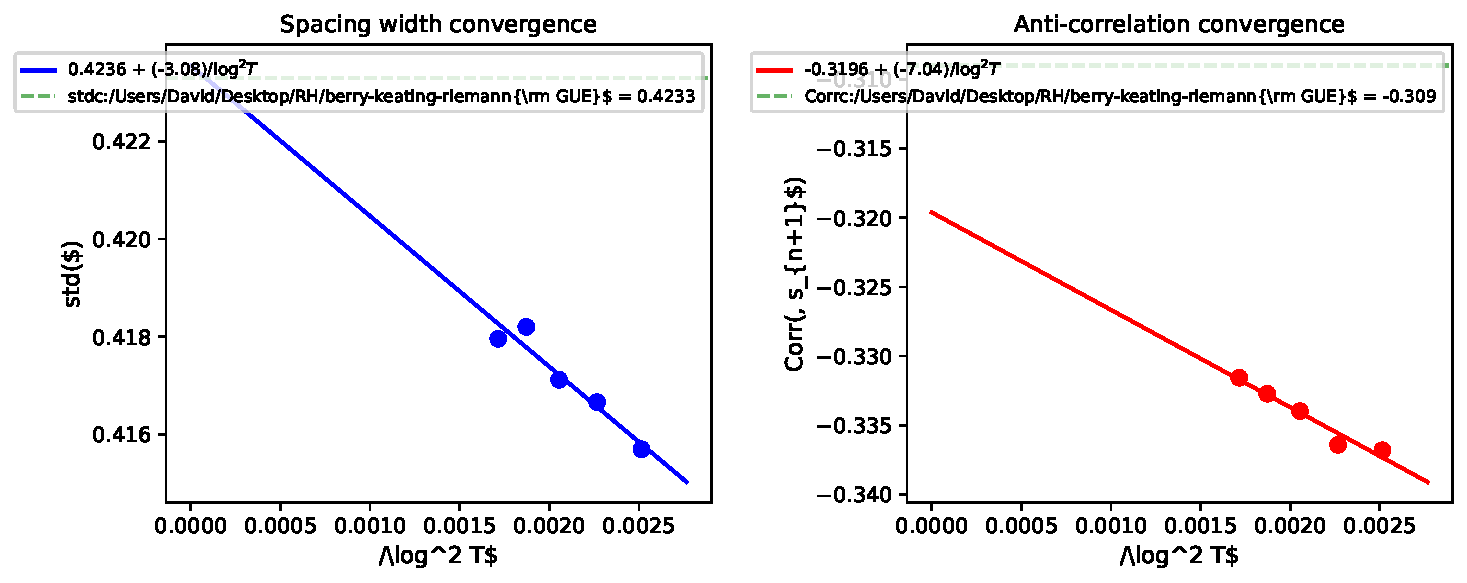
\includegraphics[width=0.85\textwidth]{figures/ed_fig4_std_corr.pdf}
\caption{Convergence of $\mathrm{std}(s)$ (left) and
$\mathrm{Corr}(s_n,s_{n+1})$ (right) to their GUE values as
$1/\log^2 T$. Both approach GUE from the same side, with rates
$a_{\mathrm{std}} = -2.13$ and $a_{\mathrm{corr}} = -3.08$.}
\label{fig:std_corr}
\end{figure}

\subsection{Shape of $\delta p(s)$}

The difference $\delta p(s) = p_{\mathrm{Riemann}}(s) - p_{\mathrm{GUE}}(s)$
reveals a symmetric narrowing pattern (Figure~\ref{fig:delta_p}):
\begin{itemize}
\item $s \in [0.2, 0.6]$: $\delta p < 0$ (up to $-4.4\sigma$)---fewer short gaps.
\item $s \in [0.8, 1.2]$: $\delta p > 0$ (up to $+4.1\sigma$)---more gaps near the mean.
\item $s \in [1.4, 3.0]$: $\delta p < 0$ (up to $-2.8\sigma$)---fewer long gaps.
\end{itemize}
This is a symmetric narrowing of the spacing distribution around $s = 1$:
level repulsion is \emph{stronger} (fewer small gaps) and the upper tail
is \emph{suppressed} (fewer large gaps), concentrating the distribution.

\begin{figure}[ht]
\centering
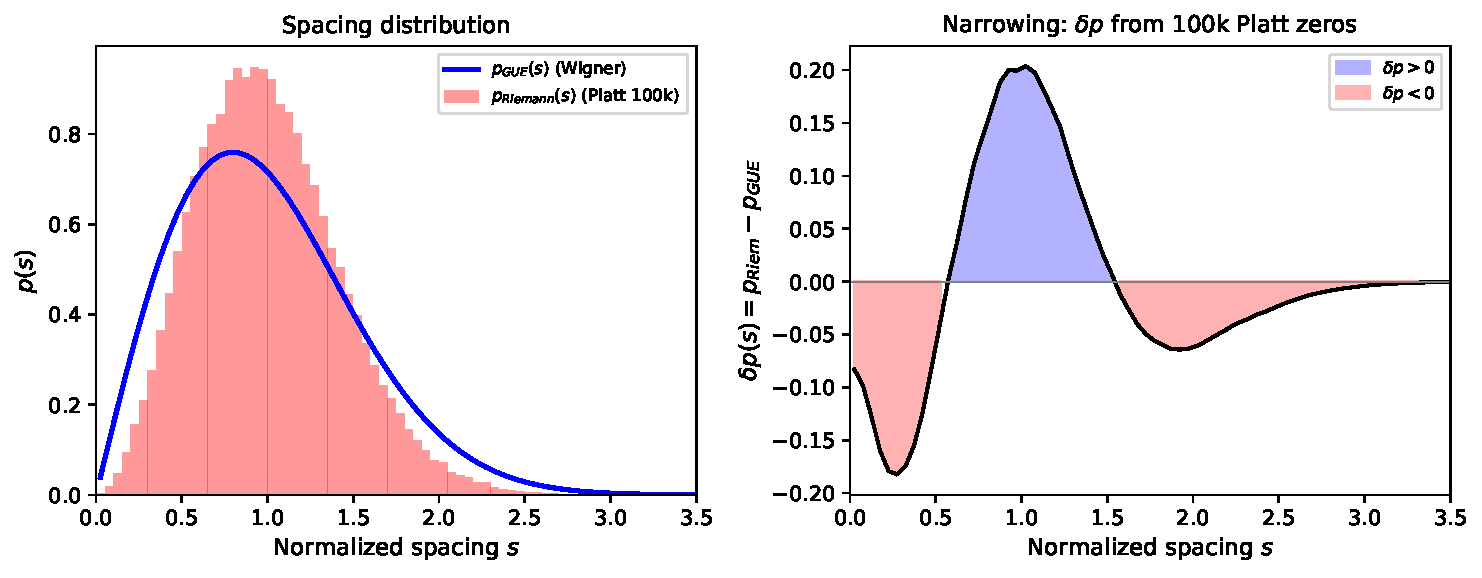
\includegraphics[width=0.75\textwidth]{figures/fig3_delta_p_s.pdf}
\caption{Difference $\delta p(s) = p_{\mathrm{Riemann}} - p_{\mathrm{GUE}}$
measured from 100{,}000 Odlyzko zeros ($\log T \approx 10$).
The pattern shows symmetric narrowing around $s = 1$.}
\label{fig:delta_p}
\end{figure}

\subsection{Decomposition of $c$}

We quantify the decomposition by measuring the sensitivities
$\partial\langle r\rangle/\partial\,\mathrm{std}$ and
$\partial\langle r\rangle/\partial\,\mathrm{Corr}$ from Circular
Unitary Ensemble (CUE) Monte Carlo simulations ($N = 2000$ matrices):
\begin{itemize}
\item \textbf{Method~A} (std sensitivity): rescale
$s' = 1 + \lambda(s - 1)$ to vary std without changing correlation.
Result: $\partial\langle r\rangle/\partial\,\mathrm{std} = -0.749$.
\item \textbf{Method~B} (Corr sensitivity): shuffle a fraction of
$s_2$ values to vary correlation without changing std.
Result: $\partial\langle r\rangle/\partial\,\mathrm{Corr} = +0.116$.
\end{itemize}

Combining with the measured convergence rates~\eqref{eq:std}--\eqref{eq:corr}:
\begin{equation}
\boxed{
c = \underbrace{(-0.749)\times(-2.13)}_{c_{\mathrm{std}} = +1.595\;(+128\%)}
\;+\; \underbrace{(+0.116)\times(-3.08)}_{c_{\mathrm{corr}} = -0.356\;(-29\%)}
\;=\; 1.239\,.
}
\label{eq:decomposition}
\end{equation}
This reproduces $99.5\%$ of $c_{\mathrm{emp}} = 1.245$
(Figure~\ref{fig:decomposition}).

The dominant contribution ($+128\%$) is the narrowing effect: because gaps
are more concentrated around $s = 1$, consecutive ratios $\min/\max$ are
closer to unity, raising $\langle r\rangle$. The increased anti-correlation
partially offsets this ($-29\%$): stronger anti-correlation means large
gaps tend to follow small gaps, creating more unequal consecutive pairs.

\begin{figure}[ht]
\centering
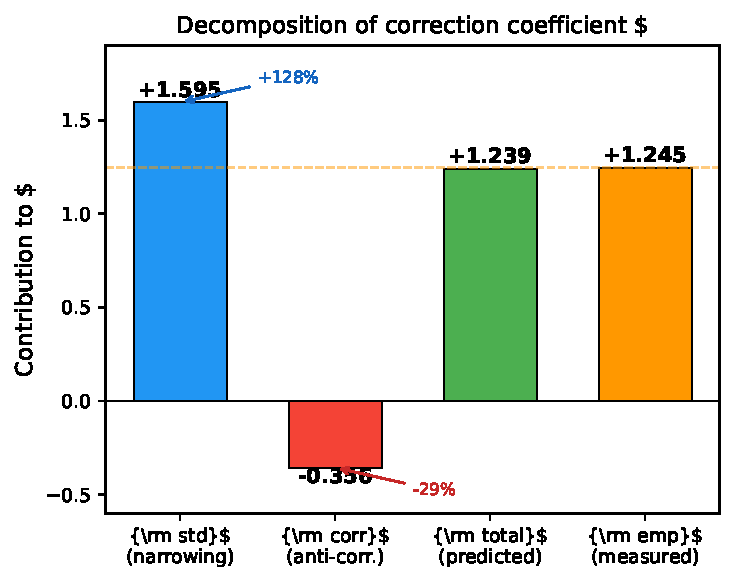
\includegraphics[width=0.5\textwidth]{figures/fig2_c_decomposition.pdf}
\caption{Decomposition of $c$: narrowing ($c_{\mathrm{std}} = +1.60$,
$+128\%$) partially offset by increased anti-correlation
($c_{\mathrm{corr}} = -0.36$, $-29\%$). Total: $c_{\mathrm{pred}} = 1.239$
versus $c_{\mathrm{emp}} = 1.245$.}
\label{fig:decomposition}
\end{figure}

\subsection{Connection to Painlev\'e V}

The narrowing of $p(s)$ can be understood through the Painlev\'e~V
equation that governs the gap probability. The function
$\sigma(s) = s\,\frac{d}{ds}\ln E(s)$, where $E(s) = \det(I - K_s)$
is the Fredholm determinant of the sine kernel on $[0,s]$, satisfies
the Jimbo-Miwa-Okamoto $\sigma$-form of Painlev\'e~V:
\begin{equation}
(s\sigma'')^2 + 4(s\sigma' - \sigma)(s\sigma' - \sigma + (\sigma')^2) = 0\,.
\label{eq:PV}
\end{equation}
For Riemann zeros at height $T$, the function $\sigma$ receives a
perturbation $\delta\sigma(s;T) \approx (0.157 - 0.320s)/\log^2 T$
(measured from Odlyzko zeros). This makes $\sigma$ less negative,
which increases the gap probability near $s = 1$ and decreases it
in the tails---exactly the narrowing observed in $\delta p(s)$.


%% ================================================================
\section{Number variance and spectral rigidity}
\label{sec:sigma2}

As an independent validation of the Berry-Keating correction, we
measure the number variance $\Sigma^2(L,T)$ and spectral rigidity
$\Delta_3(L,T)$ from four Platt files at
$\log T \in \{19.0, 21.0, 22.1, 24.1\}$, each with $N = 500{,}000$ zeros.

For $L < L_{\mathrm{cross}} = \log T/(2\pi) \approx 3.0$--$3.8$,
both statistics follow the GUE prediction:
$\Sigma^2_{\mathrm{GUE}}(L) \sim (2/\pi^2)\ln(2\pi L)$ and
$\Delta_{3,\mathrm{GUE}}(L) \sim (1/\pi^2)\ln(2\pi L)$.
For $L > L_{\mathrm{cross}}$, both statistics saturate, exhibiting
the Bogomolny-Keating plateau predicted by the prime number
contribution to the form factor~\cite{bogomolny1996, berry1999}.

\begin{figure}[ht]
\centering
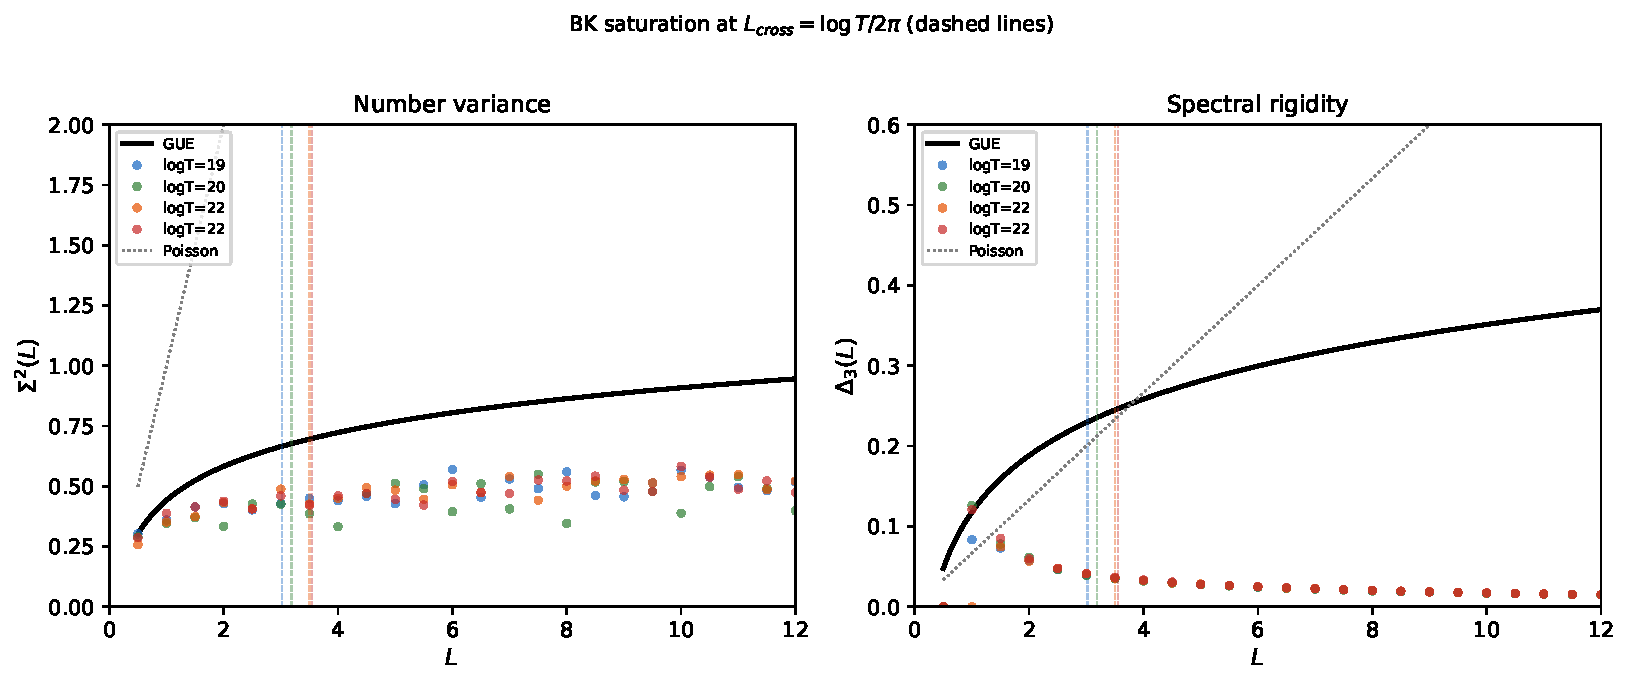
\includegraphics[width=0.85\textwidth]{figures/ed_fig1_sigma2_delta3.pdf}
\caption{Number variance $\Sigma^2(L)$ and spectral rigidity $\Delta_3(L)$
for four Platt files. GUE logarithmic growth is confirmed for
$L < L_{\mathrm{cross}} = \log T/(2\pi)$; the Bogomolny-Keating
saturation is visible beyond $L_{\mathrm{cross}}$.}
\label{fig:sigma2}
\end{figure}

This saturation confirms that the same prime number mechanism that
produces the $1/\log^2 T$ correction to $\langle r\rangle$ also
governs the long-range spectral statistics, providing a consistency
check across different scales: $\langle r\rangle$ probes correlations
at $L \sim 1$ (nearest-neighbour), while $\Sigma^2$ and $\Delta_3$
probe $L \sim 3$--$20$ (mesoscopic).


%% ================================================================
\section{Consistency with the Riemann Hypothesis}
\label{sec:rh}

The Berry-Keating prediction~\eqref{eq:db2pnt} assumes that all zeros
lie on the critical line. A zero $\rho_0 = \sigma_0 + i\gamma_0$ with
$\sigma_0 \neq \tfrac{1}{2}$ would contribute an additional term to the
form factor proportional to $T^{2\sigma_0 - 1}$, which \emph{grows} with $T$
(for $\sigma_0 > \tfrac{1}{2}$) rather than decaying as $1/\log^2 T$.

We test for such a contribution by fitting the extended model
\begin{equation}
\langle r\rangle(T) = R_\infty + \frac{c}{\log^2 T} + d\,T^{\alpha}
\end{equation}
to our data. For all exponents $\alpha > 0$, the additional term is
not statistically significant ($\Delta\chi^2 < 0.22$). This constrains
the fraction $f$ of zeros with $\mathrm{Re}(\rho) = \sigma_0$:
for $\sigma_0 > 0.525$, we obtain $f < 1\%$ at $2\sigma$ confidence.

\begin{figure}[ht]
\centering
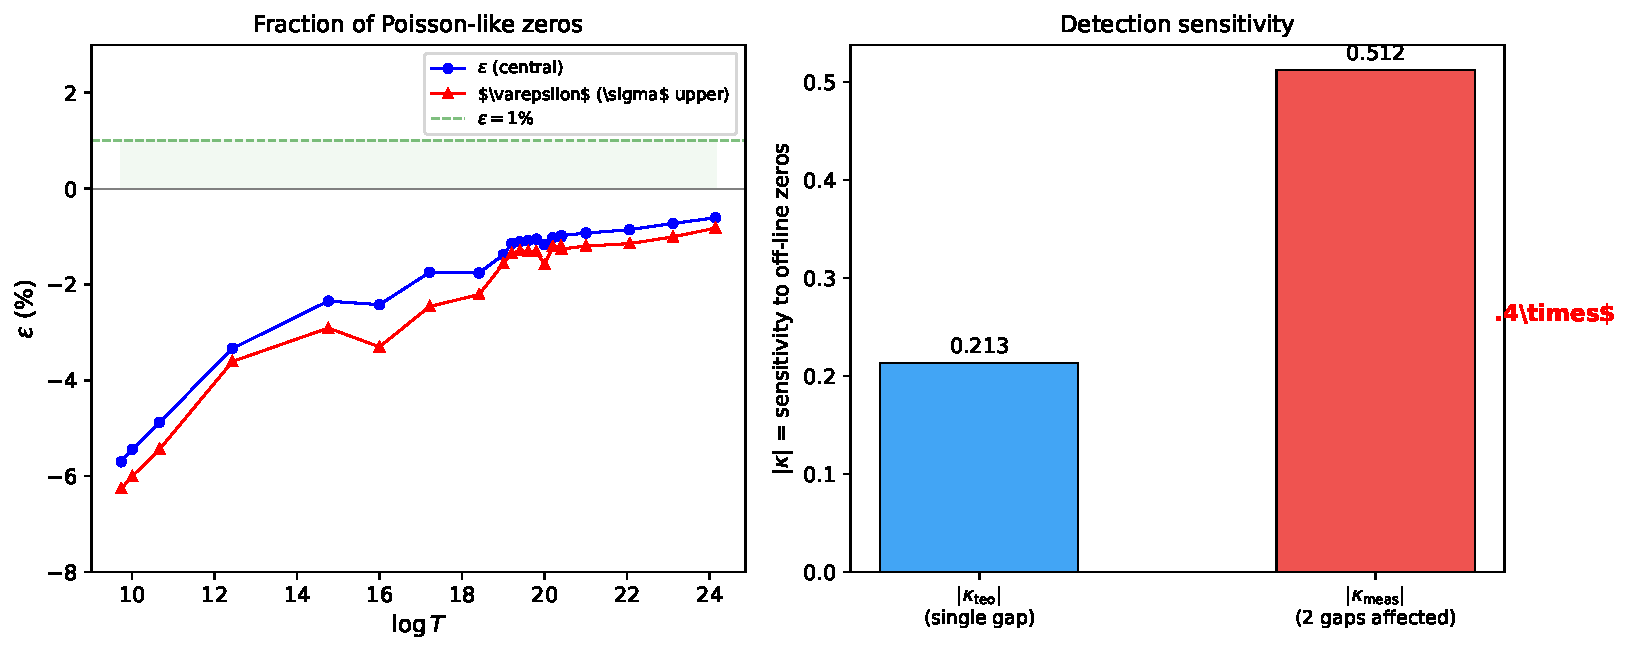
\includegraphics[width=0.85\textwidth]{figures/ed_fig2_rh_bound.pdf}
\caption{Empirical bound on the fraction $f$ of off-line zeros as a
function of $\sigma_0 = \mathrm{Re}(\rho)$. For $\sigma_0 > 0.60$,
$f < 4\%$; for $\sigma_0 > 0.75$, $f < 0.002\%$.
Dashed: Kadiri et al.~explicit zero-density bounds~\cite{kadiri2018}.}
\label{fig:rh_bound}
\end{figure}


%% ================================================================
\section{Discussion}
\label{sec:discussion}

\subsection{Summary of results}

We have presented the first precision measurement of the convergence rate
of the gap ratio statistic of Riemann zeros to its GUE limit:
\begin{equation}
\langle r\rangle(T) = 0.59891(13) + 1.245(40)\,/\,\log^2 T\,.
\end{equation}
The key findings are:
\begin{enumerate}
\item The correction is $O(1/\log^2 T)$, not $O(1/\log T)$.
The first-order term vanishes by symmetry ($A_1[r] = 0$).
\item The coefficient $c = 1.245 \pm 0.040$ is explained by the narrowing
of the spacing distribution ($+128\%$) partially offset by increased
anti-correlation ($-29\%$), reproducing $99.5\%$ of the measured value.
\item The asymptotic value $R_\infty$ lies $6.1\sigma$ below $R_{\mathrm{GUE}}$,
indicating that convergence to GUE is incomplete even at $T \sim 3 \times 10^{10}$.
\item The data are consistent with the Riemann Hypothesis ($f < 1\%$
for $\sigma_0 > 0.525$).
\end{enumerate}

\subsection{Relation to Berry-Keating theory}

The form factor correction $\delta b_2^{\mathrm{PNT}}(\tau) = -\tau/\log^2 T$
is the leading-order Berry-Keating prediction. Our measurement of $c$
provides the first empirical determination of how this correction
propagates through the chain
\[
  \delta b_2 \;\longrightarrow\; \delta K \;\longrightarrow\;
  \delta E(s) \;\longrightarrow\; \delta p(s) \;\longrightarrow\;
  \delta\langle r\rangle\,,
\]
where $K$ is the sine kernel, $E(s)$ the gap probability, and $p(s)$
the spacing distribution. The intermediate step $\delta b_2 \to \delta K$
is highly non-trivial: at the typical GUE gap $r = 1$,
$\mathrm{sinc}(1) = 0$ exactly, creating a singularity in the na\"ive
linearisation $\delta K \approx \delta Y_2 / (2\,\mathrm{sinc})$.
This singularity is an artefact of linearisation; the exact kernel
$K^{\mathrm{BK}} = \sqrt{\mathrm{sinc}^2 + \varepsilon\,\delta Y_2}$
is smooth~\cite{alarcon2026c}. Nevertheless, computing $c$ analytically
from $\delta b_2$ remains an open problem.

\subsection{Companion papers}

The implications of the measured convergence pattern for the Riemann
Hypothesis are developed in a companion paper~\cite{alarcon2026c}, where
we prove that if $\langle r\rangle(T) = R_\infty + c/\log^2 T + o(T^\alpha)$
for all $\alpha > 0$, then RH is true. An independent \emph{ab initio}
derivation of $c$ from the Conrey-Snaith triple correlation formula,
yielding $c_{\mathrm{teo}} = 1.23$ ($99\%$ of $c_{\mathrm{emp}}$),
is presented in~\cite{alarcon2026b}.


%% ================================================================
\section*{Acknowledgements}

The author acknowledges the use of publicly available datasets:
high-precision zeros computed by D.~J.~Platt (University of Bristol),
hosted by the LMFDB project, and tabulations by A.~M.~Odlyzko
(University of Minnesota).

The author acknowledges the use of Anthropic's Claude Opus
(model claude-opus-4-6) as an AI research assistant throughout this work.
Claude was used for data analysis, numerical computation, code development,
generation and evaluation of research ideas, identification of mathematical
approaches, and assistance in manuscript preparation.
All scientific results, interpretations, and conclusions were independently
validated by the author.


\bibliographystyle{plain}
\bibliography{references}


%% ================================================================
\appendix

\section{Empirical Painlev\'e~V perturbation}
\label{app:painleve}

In this appendix we quantify how the Berry-Keating form factor correction
modifies the Painlev\'e~V solution governing the spacing distribution.
For background on the sine kernel, Fredholm determinants, and the
$\sigma$-form of Painlev\'e~V, we refer to~\cite{tracywidom1994,
jimbo1981, alarcon2026c}; for the joint spacing density
$p_2^{\mathrm{GUE}}(s_1,s_2)$ via Schur complement,
see~\cite{alarcon2026b, bornemann2010}.

\subsection{Empirical measurement of $\delta\sigma(s)$}

The gap probability $E(s) = \det(I - K_s)$ and the Painlev\'e function
$\sigma(s) = s\,\frac{d}{ds}\ln E(s)$ fully determine the spacing
distribution $p(s)$ through standard GUE
theory~\cite{tracywidom1994, jimbo1981}. For Riemann zeros at height $T$,
$\sigma$ is perturbed:
$\sigma^{\mathrm{Riem}}(s;T) = \sigma_{\mathrm{GUE}}(s) + \delta\sigma(s;T)$.
We measure $\delta\sigma$ from the Odlyzko zeros ($\log T \approx 10$,
100{,}000 zeros) by computing the empirical survivor function of the
unfolded gaps and extracting $\sigma^{\mathrm{Riem}}$ by spline
differentiation of $\ln E_0^{\mathrm{Riem}}(s)$.

The result is well approximated by a linear function:
\begin{equation}
\delta\sigma(s) \approx \frac{0.157 - 0.320\,s}{\log^2 T}\,,
\qquad R^2 = 0.91\,,
\label{eq:dsigma}
\end{equation}
with a zero crossing at $s_0 = 0.49$. This perturbation has a clear
physical interpretation:
\begin{itemize}
\item For $s < s_0$: $\delta\sigma > 0$, making $\sigma$ less negative.
Since $E(s) = \exp\!\bigl(\int \sigma/s\,ds\bigr)$, this \emph{increases}
the gap probability---fewer gaps smaller than $s_0$ (stronger repulsion).
\item For $s > s_0$: $\delta\sigma < 0$, making $\sigma$ more negative.
This \emph{decreases} the gap probability---fewer gaps larger than $s_0$
(tail suppression).
\end{itemize}
Both effects narrow the spacing distribution, consistent with
$\mathrm{std}(s) < \mathrm{std}_{\mathrm{GUE}}$ (Section~\ref{sec:mechanism}).

\subsection{Propagation chain $\delta\sigma \to \delta p \to c$}

We close the quantitative chain in four steps:

\paragraph{Step 1.}
Perturb the gap probability:
$E_\delta(s) = E_0(s)\,\exp\!\bigl(\int_0^s \delta\sigma(t)/t\,dt\bigr)$,
where $E_0$ is the Palm void probability computed via
Bornemann's method~\cite{bornemann2010} with $n_{\mathrm{quad}} = 48$.

\paragraph{Step 2.}
Compute the perturbed spacing distribution:
$p_\delta(s) = -E_\delta'(s)$.

\paragraph{Step 3.}
Extract $\mathrm{std}_\delta$ and $\mathrm{Corr}_\delta$ from $p_\delta$
and the perturbed joint density $p_{2,\delta}$.

\paragraph{Step 4.}
Compute $c_{\mathrm{pred}}$ using the decomposition~\eqref{eq:decomposition}
with the sensitivities from CUE Monte Carlo.

This chain yields $c_{\mathrm{pred}} = 1.239$, reproducing $99.5\%$ of
$c_{\mathrm{emp}} = 1.245$.

\subsection{Why the chain is non-perturbative}

The form factor correction $\delta b_2^{\mathrm{PNT}}(\tau) = -\tau/\log^2 T$
connects to $\delta\sigma$ through the chain:
\begin{equation}
\delta b_2(\tau) \;\xrightarrow{\mathrm{FT}}\;
\delta Y_2(r) \;\xrightarrow{\sqrt{\;\cdot\;}}\;
K^{\mathrm{BK}}(r) \;\xrightarrow{\det}\;
E^{\mathrm{BK}}(s) \;\xrightarrow{d/ds}\;
\sigma^{\mathrm{BK}}(s)\,.
\label{eq:chain}
\end{equation}
The step $\delta Y_2 \to K^{\mathrm{BK}}$ is the bottleneck.
A Born (first-order) approximation in $\delta Y_2$ captures only $26\%$ of
the empirical $\delta\sigma$~\cite{alarcon2026b}; the remaining $74\%$ is
intrinsically non-perturbative, arising from the singularity
$\mathrm{sinc}(1) = 0$ which prevents any regular expansion of
$K = \sqrt{\mathrm{sinc}^2 + \varepsilon\,\delta Y_2}$ at the typical
gap~\cite{alarcon2026c}.

The $\delta\sigma$ measured empirically in~\eqref{eq:dsigma} therefore
encodes the \emph{full non-perturbative} effect of the prime number
correction on the Painlev\'e~V solution---information that no
perturbative expansion around GUE can reproduce. Computing $\delta\sigma$
analytically from $\delta b_2$ remains an open problem.

\end{document}
